\section*{Результаты измерений}

В работе был измерен преломляющий угол призмы $\Delta \alpha = 63^\circ 8' 35 '' \pm 0^\circ 0' 1''$.

Результаты измерений углов наименьшего отклонения $\phi$ и определённые по формуле (\ref{eq:n_lambda}) коэффициенты преломления  для спектральных линий ртути представлены в таблице. \\
\begin{tabular}{|c|c|c|c|c|c|c|c|c|}
	\hline
	Цвет & фиолетовый & синий & голубой & зелёный & желтый & желтый & красный & красный \\
	\hline
	$\lambda, \nm$ & 404,7 & 435,8 & 491,6 & 546,1 & 577,0 & 579,1 & 623,4 & 690,7 \\
	\hline
	$\varphi$ & $55^\circ17'27''$ & $54^\circ21'39''$ & $53^\circ10'55''$ & $52^\circ27'57''$ & $52^\circ7'37''$ & $52^\circ6'22''$ & $51^\circ42'45''$ & $51^\circ34'53''$ \\
	\hline
	$n$ & 1,64090 & 1,63291 & 1,62263 & 1,61630 & 1,61328 & 1,61310 & 1,60958 & 1,60840 \\
	\hline
\end{tabular}

Погрешность $n$ оценивалась по формуле $\sigma_n = \sqrt{\left(\frac{\partial f}{\partial \alpha} \sigma_\alpha\right)^2 + \left(\frac{\partial f}{\partial \delta} \sigma_\delta\right)^2}$. \\ Для всех значений $n$ погрешность косвенных измерений примерно одинакова и равна $\sigma_n = 10^{-5}$.

Построим график дисперсионной кривой $n(\lambda)$. \\
\begin{figure}[H]
	\centering
	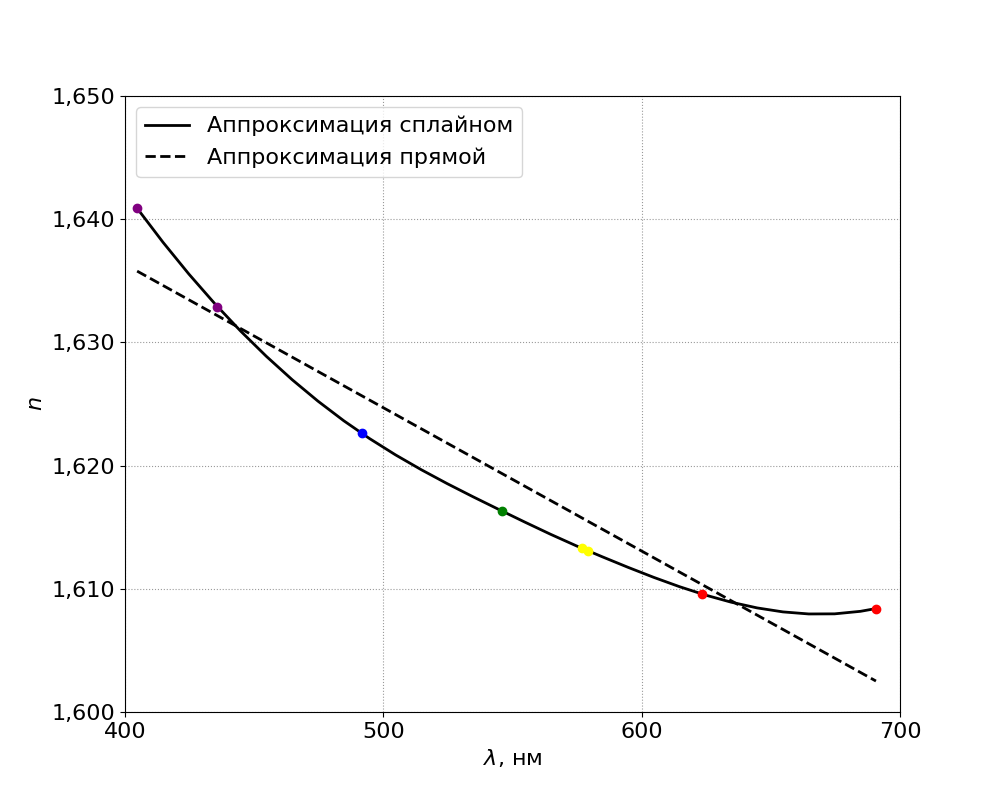
\includegraphics[width = 0.6 \textwidth]{../Графики/n(lambda).png}
\end{figure}

Согласно ГОСТ-13659-78 средняя дисперсия определяется по формуле: \\
$$
D = n_F - n_C
$$
где $n_F$ -- показатель преломления стекла для длины волны голубой спектральной линии водорода $F = 486,1 \nm$, $n_C$ -- показатель преломления стекла для длины волны красной спектральной линии водорода $C = 656,2 \nm$.

Так как теоретическая формула для зависимости $n(\lambda)$ не известна, для оценки средней дисперсии аппроксимируем зависимость сплайном. \\
$n_F = 1,6234$ \\
$n_C = 1,6081$ \\
$D = n_F - n_C = 0,015$. \\
Определим значение показателя преломления стекла для зелёной спектральной линии ртути $e = 546,1 \nm$ и жёлтой спектральной линии натрия $D = 589,3 \nm$. \\
$n_e = 1,6163$ \\
$n_D = 1,6122$. \\
Число Аббе $\nu_D = \frac{n_D - 1}{n_F - n_C} = 39,9$. \\
Определим тип стекла по ГОСТ-13659-78. Наилучшим образом характеристики исследуемого образца совпадают с материалом флинт Ф1: \\
$n_e = 1,6169$ \\
$n_D = 1,6128$ \\
$D = n_F - n_C = 0,01659$ \\
$\nu_D = 36,93$

Определим угловую дисперсию призмы по измерения координат спектральных линий жёлтой пары: \\
$D = \frac{d \varphi}{d \lambda} \approx \frac{\Delta \varphi}{\Delta \lambda} = (1,73 \pm 0,03) \cdot 10^{-4}$. \\
Разность длин волн спектральных линий $\Delta \lambda = 2,1 \nm$.
Погрешность угловой дисперсии оценим как $\varepsilon_D = \varepsilon_{\Delta \varphi} = \frac{\sqrt{2} \sigma_\varphi}{\Delta \varphi}$, где $\sigma_\varphi = 1''$ -- погрешность измерения угла.

Оценим максимальную разрешающую способность призмы в окрестности жёлтой пары спектральных линий. Разрешающая способность $R = a |\frac{d n}{d \lambda}|$ максимальна, если модуль производной $n(\lambda)$ максимален. Проведём прямую через две точки, соответствующие паре жёлтых спектральных линий, и по тангенсу угла наклона прямой оценим максимальное значение $|\frac{d n}{d \lambda}|$. \\
Длина основания призмы $a = 72 \pm 1 \mm$. \\
Максимальная разрешающая способность $R = (6,4 \pm 0,1) \cdot 10^3$. \\
Погрешность оценим как $\varepsilon_R = \varepsilon_a$.

Оценим максимальную разрешающую способность спектрального прибора, состоящего из гониометра, призмы и глаза экспериментатора. Проведём измерения ширины одной спектральной линии из жёлтой пары: \\
$\varphi_1 = 128^\circ 02' 44''$ \\
$\varphi_2 = 128^\circ 03' 03''$ \\
Считаем угловую дисперсию в области жёлтой пары спектральных линий одинаковой, тогда 
$$D = \frac{\delta \varphi}{\delta \lambda} = \frac{\Delta \varphi}{\Delta \lambda}$$
$$R = \frac{\lambda}{\delta \lambda} = \frac{\lambda}{\Delta \lambda \frac{\delta \varphi}{\Delta \varphi}}$$
где $\delta \varphi$ -- угловая ширина жёлтой спектральной линии, $\delta \lambda$ -- разность длин волн, соответствующая ширине жёлтой спектральной линии. $\Delta \varphi$ и $\Delta \lambda$ -- угловая ширина и разность длин волн для пары жёлтых спектральных линий.
$R = (1,1 \pm 0,1) \cdot 10^3$. \\
Погрешность оценим как $\varepsilon_R = \varepsilon_{\delta \lambda} = \sqrt{(\frac{\sqrt{2} \sigma_{\varphi}}{\delta \varphi})^2 + (\frac{\sqrt{2} \sigma_{\varphi}}{\Delta \varphi})^2}$.
